\section{Clustering}
El propósito en esta fase no es anticipar una etiqueta conocida, sino descubrir la estructura intrínseca y los patrones ocultos que residen en la base de datos. 

\subsection{Definición del Enfoque y Submuestreo}
Aplicar un algoritmo de agrupamiento sobre el total de la muestra (1,000,000 de registros) resultaría computacionalmente ineficiente e irrelevante para el negocio. Se adoptó la decisión de **aislar y analizar de manera exclusiva la cartera en Etapa 3 (Riesgo Alto)**. Esto se sustenten en que el incumplimiento no es un fenómeno homogéneo; las cohortes transitan hacia la cartera vencida impulsadas por diferentes combinaciones de vulnerabilidades demográficas, socioeconómicas y estructurales. Al agrupar únicamente a las observaciones deterioradas, el algoritmo responderá a una pregunta: \textit{¿Cuáles son los perfiles estructurales del incumplimiento hipotecario en México?}

A partir de la muestra de un millón de registros, de las 80,285 cohortes clasificadas en Etapa 3 (obtenidas por la partición del modelo supervisado para el conjunto de pruebas), para garantizar la viabilidad computacional en el cálculo de distancias cruzadas, se extrajo una submuestra aleatoria representativa de 10,000 registros, excluyendo la variable constante \texttt{etapa} (ya que toda esta muestra es de la Etapa 3) resultando en un vector de 9 dimensiones.

\subsubsection{Métrica de Similitud: Distancia de Gower}
La \textit{Distancia Euclidiana} es inapropiada para datos categóricos . Para solucionar esto, se implementó la \textbf{Distancia de Gower}. Esta métrica calcula una similitud parcial dependiendo de la naturaleza de cada variable: para las métricas financieras calcula diferencias absolutas estandarizadas por el rango máximo, para mitigar los atípicos; para las dimensiones categóricas, aplica un coeficiente de coincidencia binaria. La agregación de estas similitudes genera una matriz cuadrada $(10,000 \times 10,000)$ donde los valores oscilan estrictamente entre $0$ (cohortes idénticas) y $1$ (cohortes diametralmente opuestas).

\subsubsection{Algoritmo de Particionamiento: PAM (K-Medoids)}
Evaluando las alternativas algorítmicas, \textit{K-Means} fue descartado debido a su alta sensibilidad a valores atípicos y a su incapacidad para generar centroides reales y fielmente interpretables en datos categóricos. 

En su lugar, se seleccionó el algoritmo \textbf{PAM (\textit{Partitioning Around Medoids})}. PAM opera minimizando la suma de distancias absolutas a un conjunto de observaciones representativas llamadas \textit{medoides}. Su ventaja radica en la robustez frente a extremos monetarios y, críticamente, en su interpretabilidad: el centroide de cada clúster no es un promedio, sino un registro real en la base de datos.

\subsection{Determinación de Clústeres y Validación Dimensional}
Para determinar el hiperparámetro $K$ (número de grupos), se ejecutó una validación interna utilizando el \textbf{Coeficiente de Silueta} sobre la matriz de Gower precomputada.

El coeficiente evaluó la cohesión interna y la separación externa de los grupos para valores desde $K=2$ hasta $K=6$. El rendimiento máximo se alcanzó en \textbf{$K=2$}.

\begin{figure}[H]
	\centering
	\vspace{-0pt}
	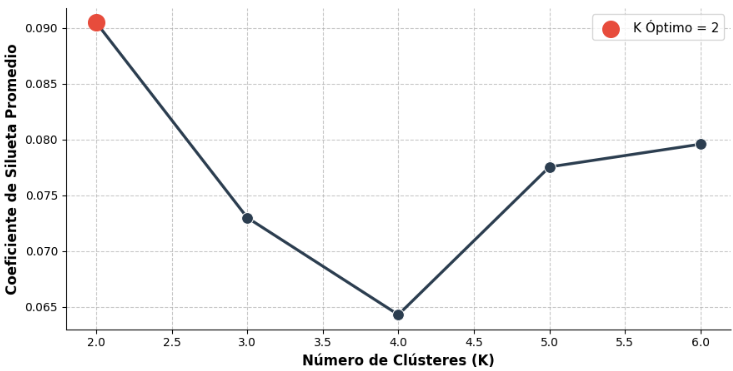
\includegraphics[scale=0.45]{imagenes/Capturas/graph-6-1.png}
	\caption{Coeficiente de Silueta evaluando distintos valores de $K$}
	\vspace{-10pt}
\end{figure}

Posterior a la partición por PAM, se aplicó una técnica de reducción de dimensionalidad no lineal, t-SNE (\textit{t-distributed Stochastic Neighbor Embedding}) a partir de la matriz de Gower para proyectar la separación de los clústeres en un espacio bidimensional, confirmando que el algoritmo logró separar la cartera vencida en dos nubes de densidad.

\begin{figure}[H]
	\centering
	\vspace{-0pt}
	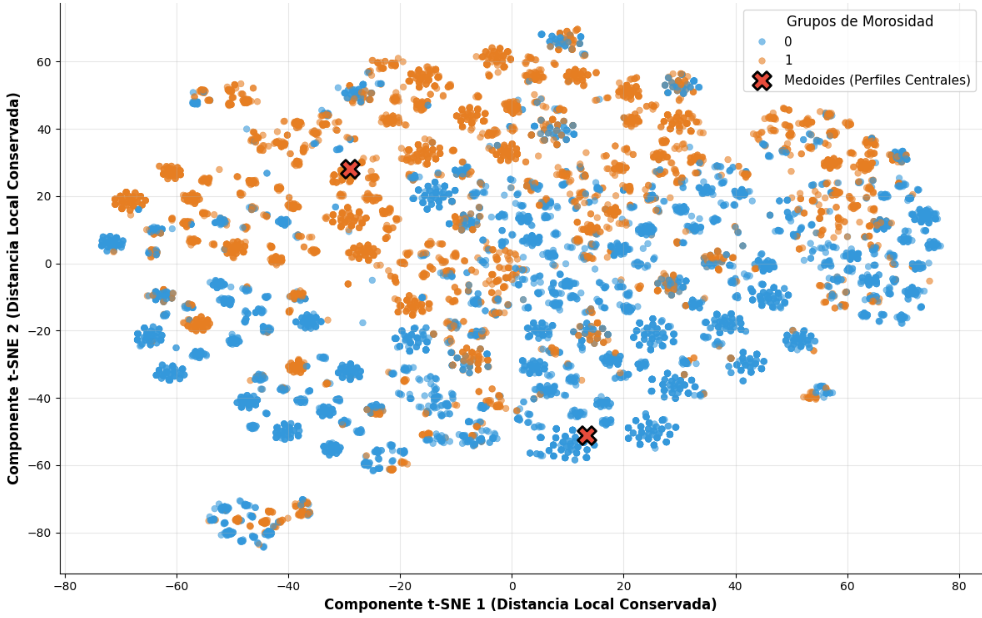
\includegraphics[scale=0.45]{imagenes/Capturas/graph-6-2.png}
	\caption{Proyección t-SNE bidimensional de los clústeres de la Etapa 3}
	\vspace{-10pt}
\end{figure}

\subsection{Interpretación de los Perfiles de Morosidad}
Para interpretar claramente los agrupamientos , se cruzaron las asignaciones del modelo PAM con el vector de características original.

Como primer análisis visual preliminar, mostrado mediante gráficos de dispersión estocástica (\textit{Stripplots}) entre edad e ingreso, insinuó patrones de agrupación en cuadrantes específicos de la matriz demográfica. Sin embargo, para cuantificar las fronteras de manera más completa e integra, se recurrió al análisis de frecuencias de las dimensiones categóricas estructurales.

\begin{figure}[H]
	\centering
	\vspace{-0pt}
	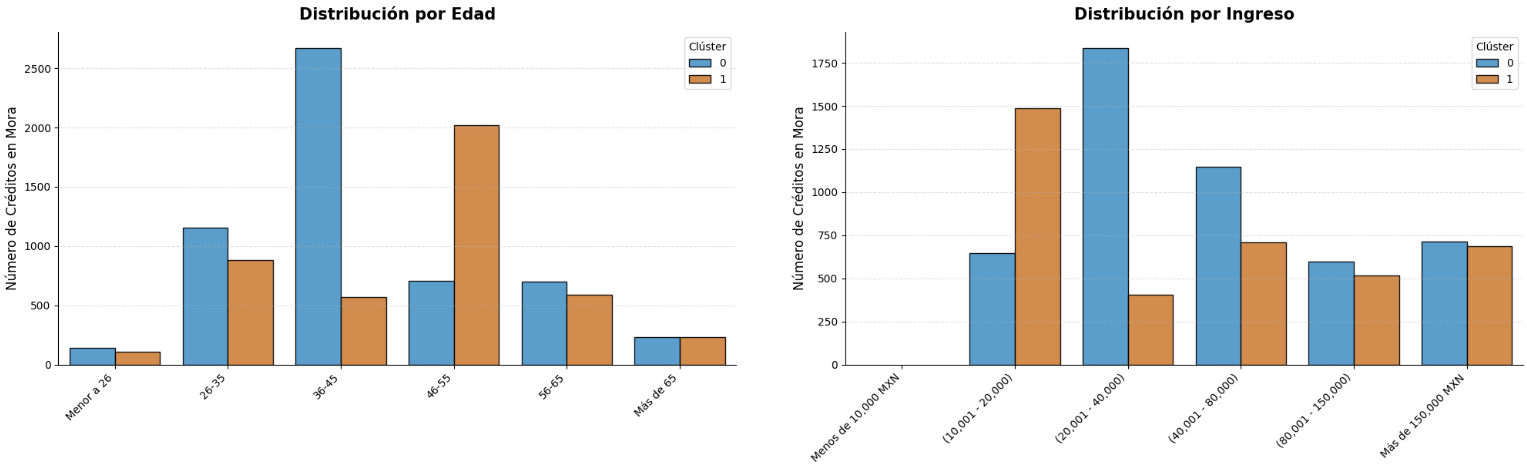
\includegraphics[scale=0.32]{imagenes/Capturas/graph-6-3.png}
	\vspace{-10pt}
\end{figure}
\begin{figure}[H]
	\centering
	\vspace{-0pt}
	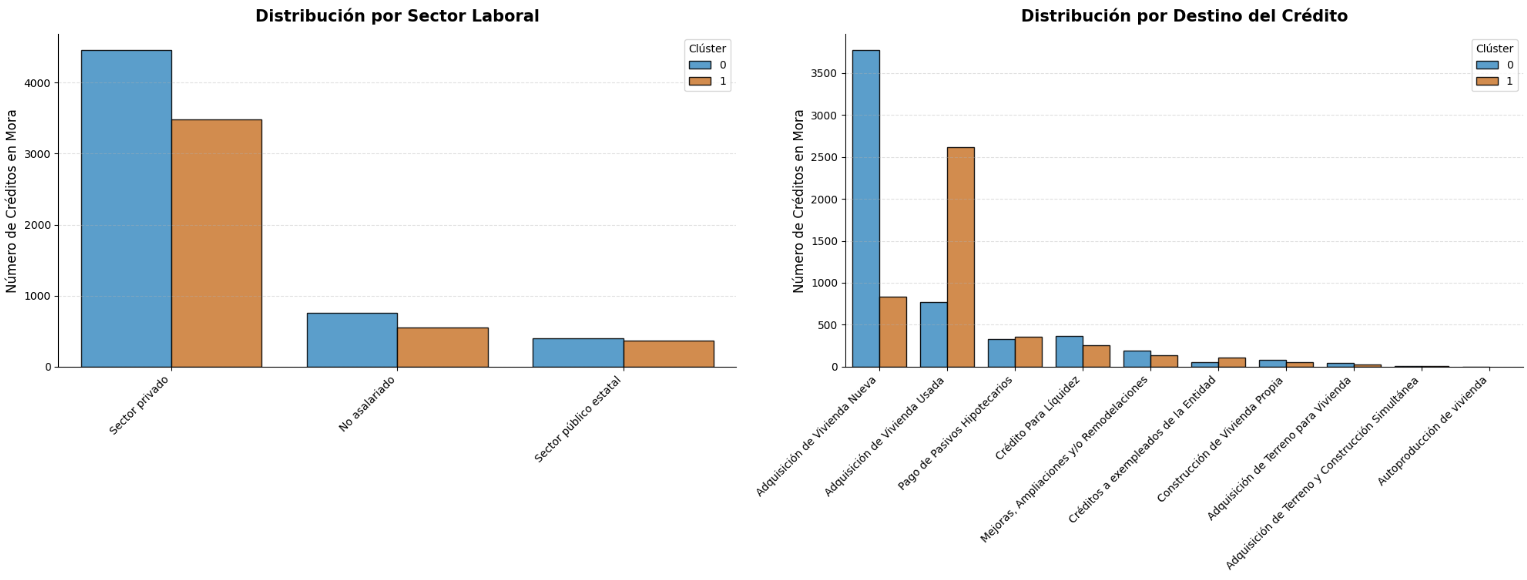
\includegraphics[scale=0.32]{imagenes/Capturas/graph-6-4.png}
	\vspace{-10pt}
\end{figure}
\begin{figure}[H]
	\centering
	\vspace{-0pt}
	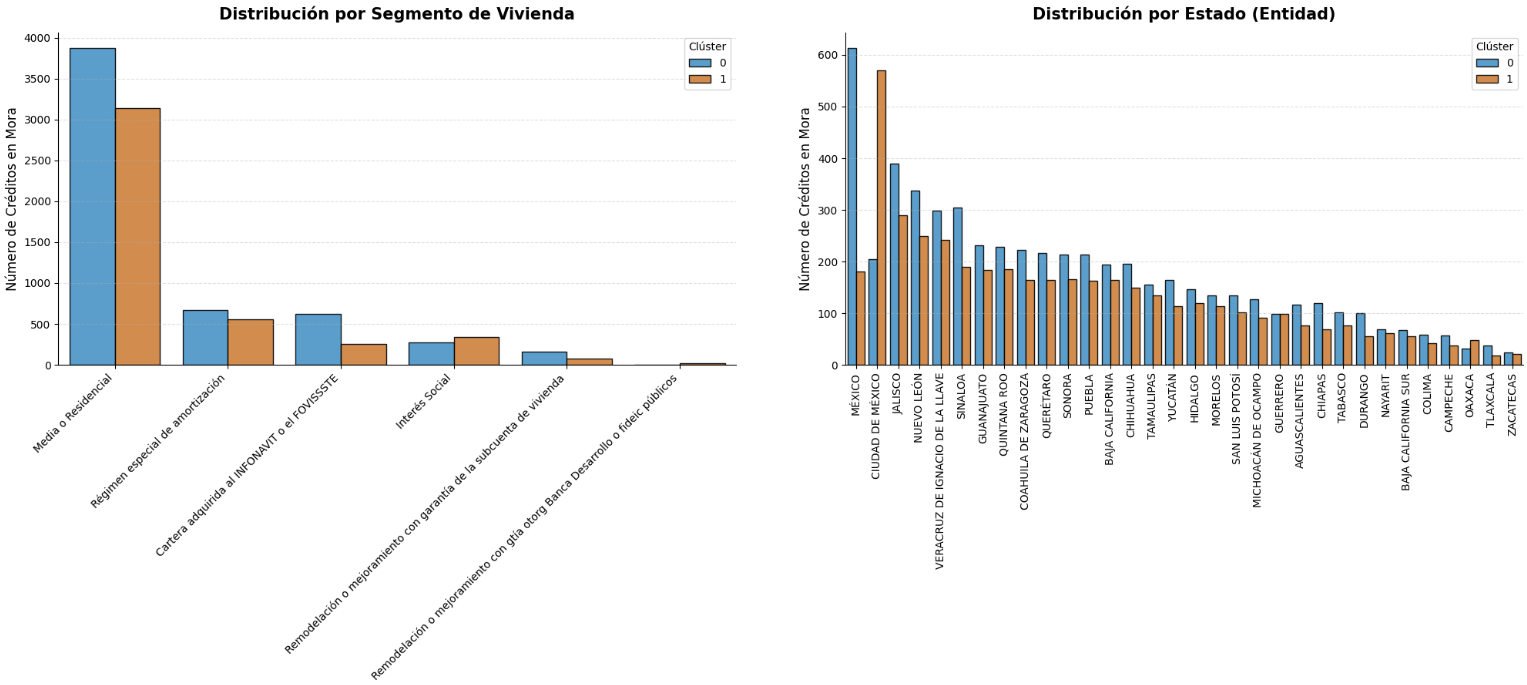
\includegraphics[scale=0.32]{imagenes/Capturas/graph-6-5.png}
	\caption{Distribución de los clústeres de la Etapa 3 en las variables catégoricas}
	\vspace{-10pt}
\end{figure}

La convergencia de estos análisis visuales con la identidad financiera de los medoides revelados por el algoritmo, reveló formalmente los dos principales perfiles que originan el deterioro crediticio:

\begin{itemize}
	\item \textbf{Perfil 0:} \\
	Agrupa a cohortes en una etapa de madurez media (36-45 años) con ingresos medios-altos (\$20,001 a \$40,000 MXN). El deterioro surge en operaciones destinadas a la \textit{Adquisición de Vivienda Nueva}, típicamente ubicadas en la periferia de crecimiento urbano continuo (como el Estado de México). Presentan deudas conjuntas moderadas (mediana cercana a los \$754,566 MXN) a tasas estandarizadas (10.75\%). 
	
	\item \textbf{Perfil 1:} \\
	Agrupa a cohortes en etapas de mayor madurez (46-55 años) y con una ingresos inferiores (\$10,001 a \$20,000 MXN). El incumplimiento en este estrato se acentúa en \textit{Adquisición de Vivienda Usada}, concentrándose fuertemente en el centro del país (Ciudad de México). Contraintuitivamente a sus ingresos, las cohortes de este grupo sostienen niveles de deuda conjuntas muy elevados (mediana superior a \$1.3 millones MXN) a tasas ligeramente preferenciales (10.00\%). 
\end{itemize}

\subsection{Conclusión del Análisis Descriptivo}
El modelo no supervisado dotó perfiló el concepto de riesgo alto. Mientras que las redes neuronales operan como predictores de riesgo, el agrupamiento con K-Medoids indentifico la estructura que toma la cartera vencida. Al revelar que las carteras deterioradas no son uniformes, las instituciones pueden implementar estrategias especializadas (por ejemplo, esquemas de refinanciamiento temporal para el Perfil 0, o apoyos para liquidaciones para el Perfil 1), optimizando las pérdidas y recuperando liquidez.